\section{Evaluation}
\label{sec:results}

Next, we describe the data we used to train the models required to extract the features, the training of the classifier, and the results of our submission.

\subsection{Computation of features}

We need to generate two types of models to extract our features: probabilistic lexicons and language models. We used the probabilistic lexicons that can be obtained as a sub product of the training of full statistical models. In particular, we used Moses~\cite{Moses} on its default configuration with the News Commentary V13 parallel corpus as provided for the News translation shared task. We used the same corpora to train the language models. In this case, we used Kenlm~\cite{Kenlm} and estimated models of order $5$.


\subsection{Training the classifier}

We trained the classifier using again the News Commentary parallel corpus. We generate as many negative examples as positive sentence pairs in the corpus for a total of almost $600$k data points to train our classifier. The negative examples were evenly distributed among the thee perturbation operations described in the previous section. We used scikit-learn to train our gradient boosting classifier. The final trained model is used to score all sentences in the noisy corpus.

We perform some initial experiments using the Common Crawl corpus, under the rationale that it would be closer to the domain of the noisy data belonging to the Paracrawl corpus. However, Common Crawl data has quite a large number of misaligned sentences. This will result in positive data points that in reality were negative which will hinder the learning process of the classifier. We tried an iterative cleaning process so that we were not so reliant in clean, perfectly align data. However, we had to stop exploring this direction due to time constraints.


%https://docs.google.com/spreadsheets/d/1SKMOBbH5YVsQJpbUCMN3K8Gzt_89zBabQl716Aw8NjM/edit?usp=sharing
\begin{figure}[ht]
  \centering
  \begin{subfigure}[b]{\columnwidth}
    \hspace*{-1.5em}
    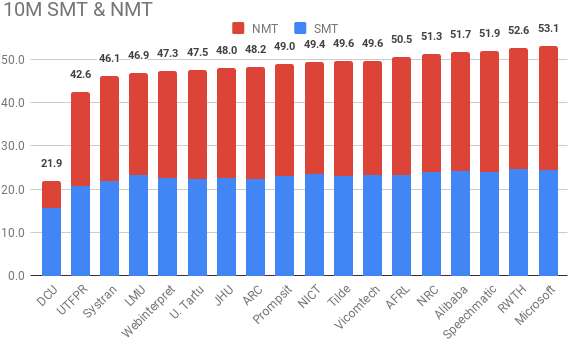
\includegraphics[width=1.1\textwidth]{images/10M_crop.png}
    \label{fig:10M}
  \end{subfigure}
  ~
  \begin{subfigure}[b]{\columnwidth}
    \hspace*{-1.5em}
    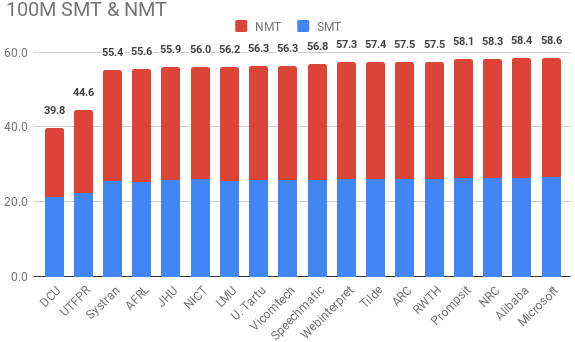
\includegraphics[width=1.1\textwidth]{images/100M_crop.png}
    \label{fig:100M}
  \end{subfigure}
  \caption{Best submission of each participant institution. We display Bleu [\%] results stacked for SMT (\textcolor{blue}{blue}) and NMT (\textcolor{red}{red}).}
  \label{fig:results}
\end{figure}

\subsection{Results}
TBA
